\documentclass[a4paper,12pt]{article}

\documentclass[a4paper,12pt]{article}

%%% Работа с русским языком
\usepackage{cmap}					% поиск в PDF
\usepackage{mathtext} 				% русские буквы в формулах
\usepackage[T2A]{fontenc}			% кодировка
\usepackage[utf8]{inputenc}			% кодировка исходного текста
\usepackage[russian,english]{babel}	% локализация и переносы
\usepackage{indentfirst}            % красная строка в первом абзаце
\frenchspacing                      % равные пробелы между словами и предложениями

%%% Дополнительная работа с математикой
\usepackage{amsmath,amsfonts,amssymb,amsthm,mathtools} % пакеты AMS
\usepackage{icomma}                                    % "Умная" запятая

%%% Свои символы и команды
\usepackage{centernot} % центрированное зачеркивание символа
\usepackage{stmaryrd}  % некоторые спецсимволы

\usepackage{ifthen}

\renewcommand{\epsilon}{\ensuremath{\varepsilon}}
\renewcommand{\phi}{\ensuremath{\varphi}}
\renewcommand{\kappa}{\ensuremath{\varkappa}}
\renewcommand{\le}{\ensuremath{\leqslant}}
\renewcommand{\leq}{\ensuremath{\leqslant}}
\renewcommand{\ge}{\ensuremath{\geqslant}}
\renewcommand{\geq}{\ensuremath{\geqslant}}
\renewcommand{\emptyset}{\ensuremath{\varnothing}}

\DeclareMathOperator{\sgn}{sgn}
\DeclareMathOperator{\ke}{Ker}
\DeclareMathOperator{\im}{Im}
\DeclareMathOperator{\re}{Re}

\newcommand{\N}{\mathbb{N}}
\newcommand{\Z}{\mathbb{Z}}
\newcommand{\Q}{\mathbb{Q}}
\newcommand{\R}{\mathbb{R}}
\newcommand{\Cm}{\mathbb{C}}
\newcommand{\F}{\mathbb{F}}
\newcommand{\id}{\mathrm{id}}

\newcommand{\imp}[2]{
	(#1\,\,$\ra$\,\,#2)\,\,
}
\newcommand{\System}[1]{
	\left\{\begin{aligned}#1\end{aligned}\right.
}
\newcommand{\Root}[2]{
	\left\{\!\sqrt[#1]{#2}\right\}
}

\renewcommand\labelitemi{$\triangleright$}

\let\bs\backslash
\let\Lra\Leftrightarrow
\let\lra\leftrightarrow
\let\Ra\Rightarrow
\let\ra\rightarrow
\let\La\Leftarrow
\let\la\leftarrow
\let\emb\hookrightarrow

%%% Перенос знаков в формулах (по Львовскому)
\newcommand{\hm}[1]{#1\nobreak\discretionary{}{\hbox{$\mathsurround=0pt #1$}}{}}

%%% Работа с картинками
\usepackage{graphicx}    % Для вставки рисунков
\setlength\fboxsep{3pt}  % Отступ рамки \fbox{} от рисунка
\setlength\fboxrule{1pt} % Толщина линий рамки \fbox{}
\usepackage{wrapfig}     % Обтекание рисунков текстом

%%% Работа с таблицами
\usepackage{array,tabularx,tabulary,booktabs} % Дополнительная работа с таблицами
\usepackage{longtable}                        % Длинные таблицы
\usepackage{multirow}                         % Слияние строк в таблице

%%% Теоремы
\theoremstyle{plain}
\newtheorem{theorem}[equation]{Theorem}
\newtheorem{lemma}[equation]{Lemma}
\newtheorem{proposition}[equation]{Proposition}
\newtheorem*{exercise}{Exercise}
\newtheorem*{problem}{Problem}

\theoremstyle{definition}
\newtheorem{definition}[equation]{Definition}
\newtheorem*{corollary}{Corollary}
\newtheorem*{note}{Note}
\newtheorem*{reminder}{Reminder}
\newtheorem*{example}{Example}

\theoremstyle{remark}
\newtheorem*{solution}{Solution}

%%% Оформление страницы
\usepackage{extsizes}     % Возможность сделать 14-й шрифт
\usepackage{geometry}     % Простой способ задавать поля
\usepackage{setspace}     % Интерлиньяж
\usepackage{enumitem}     % Настройка окружений itemize и enumerate
\setlist{leftmargin=25pt} % Отступы в itemize и enumerate

\geometry{top=25mm}    % Поля сверху страницы
\geometry{bottom=30mm} % Поля снизу страницы
\geometry{left=20mm}   % Поля слева страницы
\geometry{right=20mm}  % Поля справа страницы

\setlength\parindent{0pt}         % Устанавливает длину красной строки 0pt
\linespread{1.3}                  % Коэффициент межстрочного интервала
%\setlength{\parskip}{0.5em}      % Вертикальный интервал между абзацами
%\setcounter{secnumdepth}{0}      % Отключение нумерации разделов
%\setcounter{section}{-1}         % Нумерация секций с нуля
\usepackage{multicol}			  % Для текста в нескольких колонках
\usepackage{soulutf8}             % Модификаторы начертания

%%% Содержаниие
\usepackage{tocloft}
\tocloftpagestyle{main}
%\setlength{\cftsecnumwidth}{2.3em}
%\renewcommand{\cftsecdotsep}{1}
%\renewcommand{\cftsecpresnum}{\hfill}
%\renewcommand{\cftsecaftersnum}{\quad}

%%% Шаблонная информация для титульного листа
\newcommand{\CourseName}{Introduction to Calculus}
\newcommand{\FullCourseNameFirstPart}{\so{INTRODUCTION TO CALCULUS}}
\newcommand{\SemesterNumber}{I}
\newcommand{\LecturerInitials}{Nikolay Gusev}
\newcommand{\CourseDate}{fall 2022}
\newcommand{\AuthorInitials}{Danil Klishch}
\newcommand{\VKLink}{https://vk.com/dan.klishch}
\newcommand{\GithubLink}{https://github.com/daniild71r/lectures_tex_club}

%%% Колонтитулы
\usepackage{titleps}
\newpagestyle{main}{
	\setheadrule{0.4pt}
	\sethead{\CourseName}{}{\hyperlink{intro}{\;Back to table of contents}}
	\setfootrule{0.4pt}                       
	\setfoot{MIPT, \CourseDate}{}{\thepage} 
}
\pagestyle{main}

%%% Нумерация уравнений
\makeatletter
\def\eqref{\@ifstar\@eqref\@@eqref}
\def\@eqref#1{\textup{\tagform@{\ref*{#1}}}}
\def\@@eqref#1{\textup{\tagform@{\ref{#1}}}}
\makeatother                      % \eqref* без гиперссылки
\numberwithin{equation}{subsection}  % Нумерация вида (номер_секции).(номер_уравнения)
\mathtoolsset{showonlyrefs=false} % Номера только у формул с \eqref{} в тексте.

%%% Гиперссылки
\usepackage{hyperref}
\usepackage[usenames,dvipsnames,svgnames,table,rgb]{xcolor}
\hypersetup{
	unicode=true,            % русские буквы в раздела PDF
	colorlinks=true,       	 % Цветные ссылки вместо ссылок в рамках
	linkcolor=black!15!blue, % Внутренние ссылки
	citecolor=green,         % Ссылки на библиографию
	filecolor=magenta,       % Ссылки на файлы
	urlcolor=NavyBlue,       % Ссылки на URL
}

%%% Графика
\usepackage{tikz}        % Графический пакет tikz
\usepackage{tikz-cd}     % Коммутативные диаграммы
\usepackage{tkz-euclide} % Геометрия
\usepackage{stackengine} % Многострочные тексты в картинках
\usetikzlibrary{angles, babel, quotes}

%%% Мои кастомные команды
\newcommand{\df}[2]{\begin{definition}\textit{#1} -- #2\end{definition}}

\newcommand{\abs}[1]{\left\lvert #1 \right\rvert}
\newcommand{\grad}{\mathrm{grad}\:}
\newcommand{\dlta}{\text{d}}
\newcommand{\thus}{\;\Rightarrow\;}
\newcommand{\isconst}{=\text{const}}

\newcommand{\defeq}{\vcentcolon=}
\newcommand{\defev}{\stackrel{\Delta}{\Longleftrightarrow}}
\newcommand{\deriv}[3][1]{%
	\ifthenelse{#1>1}{%
		\frac{\dlta^{#1} {#2}}{\dlta {#3}^{#1}}
	}{%
		\frac{\dlta {#2}}{\dlta {#3}}
	}%
}
\newcommand{\vc}[3]{
	\ensuremath{\begin{pmatrix} #1 \\ #2 \\ #3 \end{pmatrix}}
}
\newcommand{\vb}[2]{
	\ensuremath{\begin{pmatrix} #1 \\ #2 \end{pmatrix}}
}
\newcommand{\fnis}[1]{#1{:}\;}
\newcommand{\RR}{\mathbb{R}}
\newcommand{\NN}{\mathbb{N}}
\newcommand{\sconstr}{\;\vert\;}
\newcommand{\diag}{{\rm diag}}

\newcommand{\floor}[1]{\left\lfloor#1\right\rfloor}
\newcommand{\ceil}[1]{\left\lceil#1\right\rceil}


%%% Всю шаблонную информацию можно менять тут
\newcommand{\FullCourseNameFirstPart}{\so{ТЕОРИЯ И РЕАЛИЗАЦИЯ}}
\newcommand{\FullCourseNameSecondPart}{\so{ЯЗЫКОВ ПРОГРАММИРОВАНИЯ}}
\newcommand{\SchoolName}{ФПМИ}
\newcommand{\TrackName}{МФ}
\newcommand{\SemesterNumber}{III}
\newcommand{\LecturerInitials}{Рубцов Александр Александрович}
\newcommand{\AutherInitials}{Моложавенко Александр}
\newcommand{\VKLink}{https://vk.com/}
\newcommand{\OverleafLink}{https://www.overleaf.com/}
\newcommand{\GithubLink}{https://github.com}
\newcommand{\CourseName}{Краткое Название} %  Используется в преамбуле для создания названия предмета в верхнем контитуле   
\newcommand{\CourseDate}{Осень 2020}           %  Используется в преамбуле для создания даты в нижнем контитуле и в title_page

%\includeonly{lectures/lect05,lectures/lect06}  % Чтобы скомпилировать только часть лекций

\begin{document}
\begin{titlepage}
	\clearpage\thispagestyle{empty}
	\centering
	
	\textit{Федеральное государственное автономное учреждение \\
		высшего образования}
	\vspace{0.5ex}
	
	\textbf{Московский физико-технический институт
    \\
    (национальный исследовательский университет)
    \\
     КЛУБ ТЕХА ЛЕКЦИЙ}
	\vspace{20ex}
	
	\rule{\linewidth}{0.5mm}
	{\textbf{\FullCourseNameFirstPart}}
	\\
	{\textbf{\FullCourseNameSecondPart}}
	\rule{\linewidth}{0.5mm}
	
	\SemesterNumber\ СЕМЕСТР
	\\
	Физтех-школа: \textit{\SchoolName}
	\\
	Направление: \textit{\TrackName}
	\\
	Лектор: \textit{\LecturerInitials}
	\vspace{1ex}
	
	\begin{figure}[!ht]
		\centering
		\includegraphics[width=0.6\textwidth]{logo_LTC}
	\end{figure}
\begin{flushright}
	\noindent
	Автор(ы): \href{\VKLink}{\textit{\AutherInitials}}
	\\
	\href{\OverleafLink}{\textit{Проект на overleaf}}
	\\
	\href{\GithubLink}{\textit{Проект на github}} 
\end{flushright}
	
	\vfill
	Долгопрудный, \CourseDate\ год.
	\pagebreak
	
\end{titlepage}
\newpage
\hypertarget{intro}{}
\tableofcontents

\newpage
\begin{flushright}
    \textit{Лекция 1 (от 07.09)}
\end{flushright}
\section{$\S 1.$ Комплексные числа}
\Def
Пусть $z = \left( x;y \right) \in \RR^2$. Пусть определены операции:
\begin{enumerate}
    \item \textbf{Сложение:} $z_1 + z_2 = \left( x_1+x_2; y_1+y_2 \right)$
    \item \textbf{Умножение на действительное число:} $\lambda z = \left(\lambda
        x, \lambda y \right)$
    \item \textbf{Расстояние:} $\rho(z_1, z_2) = \left| \left| z_1 - z_2 \right|
    \right| = \sqrt{\left( x_1 - x_2 \right)^2 + (y_1 - y_2)^2}$
\end{enumerate}
Добавим операцию
умножения друг на друга:
\begin{align*}
  & z_1 \cdot z_2 = \left( x_1 \cdot x_2 - y_1 \cdot y_2; x_1 \cdot y_2 + x_2 \cdot y_1 \right)
\end{align*}
Будем называть это \textbf{комплексными числами} $\CC$.
\\
Пусть $1 \sim (1; 0)$~--- \textbf{единица}, $i \sim (0;1)$~--- \textbf{мнимая
  единица}.
\\
Тогда $z = 1 \cdot x + i \cdot y \Leftrightarrow z = x + iy$~---
\textbf{алгебраическая запись}.
\\
Назовем $x = \Real z$ \textbf{действительной частью}, $y =
\Img z$~--- \textbf{мнимой}.
\\
\textbf{Сопряженным} к $z = x+iy$ называем $\bar{z} = x-iy$,
\textbf{модулем}~--- выражение $\left| z \right| = \sqrt{x^2+y^2}$. Легко
видеть, что $z\bar{z} = \left| z \right|^2$, полагая $i^2 = -1$.
\\
Можно представлять комплексные числа в виде $x = r \cos \varphi$, $y = r \sin
\varphi$, называя $r$ \textbf{модулем}, $\varphi$ \textbf{аргументом}, а $\arg z
\in (-\pi; \pi]$~--- одно из таких $\varphi$~--- \textbf{главным аргументом}.
Также \textbf{аргументом} называется множество $\Arg z = \left\{ \arg z + 2\pi k
    \mid k \in \ZZ \right\}$.
\\
Видим, что
\begin{align*}
  & z = \left| z \right|\cos \varphi + i \left| z \right|\sin \varphi = \left| z \right|\left( \cos \varphi + i \sin \varphi \right)
\end{align*}
Введем \textbf{комплексную экспоненту}~--- $e^{i\varphi} = \cos \varphi + i \sin
\varphi$, тогда $z = \left| z \right|e^{i\varphi}$.
\\
Для произведения тогда выполняется
\begin{align*}
  & z_1z_2 = \left| z_1 \right|\left( \cos \varphi_1 + i \sin \varphi_2 \right)\left| z_2 \right|\left( \cos \varphi_2 + i \sin \varphi_2 \right) = \left| z_1 \right|\cdot \left| z_2 \right| \left( \cos \left( \varphi_1+\varphi_2 \right) + i \sin \left( \varphi_1+\varphi_2 \right)\right)
\end{align*}
\begin{align*}
  & \left|z_1z_2\right| = \left| z_1 \right|\cdot \left| z_2 \right|
\end{align*}
\begin{align*}
  & \Arg(z_1z_2) = \Arg z_1 + \Arg z_2
\end{align*}
\textbf{Суммой Минковского} называется множество $A+B = \sets{a+b \mid a\in A, \
  b \in B}$.
\\
На комплексных числах определено \textbf{деление} на $z\neq 0$: $z_1z = z_2
\Rightarrow z = \dst \frac{z_2}{z_1}$; если $z_2=1$, то $z = \dst \frac{1}{z_1}
= z_1^{-1}$.
\\
Нахождение частного эквивалентно решению системы
\begin{align*}
  & \left\{ \begin{matrix}
          x_1x-y_1y=x_2 \\
          y_1x+x_1y = y_2
      \end{matrix} \right.
\end{align*}
Это можно выразить как
\begin{align*}
  & z = \frac{\bar{z_1}z_2}{\left| z_1 \right|^2} = \frac{\left| z_2 \right|e^{i \varphi_2}}{\left| z_1 \right| e^{i \varphi_1}} = \frac{\left| z_2 \right|}{\left| z_1 \right|}e^{i\left( \varphi_2-\varphi_1 \right)}
\end{align*}
Зная, что $e^{i \varphi_1}e^{i \varphi_2} = e^{i\left( \varphi_1+\varphi_2
  \right)}$, можем записать \textbf{формулу Муавра}:
\begin{align*}
  & \forall n \in \NN \ z^n = \left| z \right|^ne^{i n \varphi} 
\end{align*}
Также определена операция \textbf{извлечения корня} из $z^n = a \neq 0$.
Полагаем $z=re^{i\varphi}$, $a = \left| a \right|e^{i\alpha}$. Тогда $r^n =
\left| \alpha \right|$, а $n \varphi = \alpha + 2 \pi k, \ k \in \ZZ$. Отсюда $r
= \sqrt[n]{\left| a \right|}$, $\varphi_k = \dst \frac{\alpha+2\pi k}{n}$. тогда
определим корень как
\begin{align*}
  & \sets{\sqrt[n]{a}} = \sets{\sqrt[n]{\left| a \right|}\left( \cos \frac{\alpha + 2 \pi k}{n} + i \sin \frac{\alpha + 2 \pi k}{n} \right)\mid k \in \{0, \dots, n-1\}}
\end{align*}
\Example
\begin{align*}
  & \sets{\sqrt[4]{i}} = \sets{\exp\left( i \frac{\dst \frac{\pi}{2} + 2 \pi k}{4} \right)\mid k \in \{0, \dots, 3\}}
\end{align*}
\section{$\S 2.$ Последовательность. Предел. Ряды. Функции. Расширенная
  комплексная плоскость}
\Def
\textbf{Окрестностью} назовем $B_r(z_0) = \left\{ z \in \CC: \left| z-z_0
    \right| < r \right\}$. \textbf{Проколотой окрестностью} назовем
$\os{\circ}{B}_r(z_0) = \left\{ z \in \CC: 0 < \left| z-z_0 \right| < r
\right\}$. \textbf{Замкнутой окрестностью} назовем $\bar{B}_r(z_0) = \left\{ z
    \in \CC: \left| z-z_0\right| \leq r \right\}$.
\Def
Множество $\left\{ z_n \right\}_{n=1}^\infty$, $z_n  = x_n + iy_n$ называется
\textbf{последовательностью}.
\Def
Число $A \in \CC$ называется \textbf{пределом последовательности $z_n$} (пишем
$\dst \lim_{n \to \infty}z_n = A$) тогда и только тогда, когда выполняется
\begin{equation}\label{(2.1)}
    \forall \varepsilon > 0 \ \exists N(\varepsilon):\ \forall n \geq N(\varepsilon)\in \NN \hookrightarrow z_n \in B_{\varepsilon}(A)
\end{equation}
\asm
\begin{align*}
  & \exists \lim_{n \to \infty}z_n = A = a+ib \Leftrightarrow \left\{ \begin{matrix}
          \dst \lim_{n \to \infty}x_n = a \\
          \dst \lim_{n \to \infty}y_n = b
      \end{matrix} \right.
\end{align*}
\pr Докажем в обе стороны.
\begin{itemize}
    \item $\Rightarrow$:
    \begin{align*}
      & \left| x_n - a \right| \leq \left| z_n - A \right| < \varepsilon
    \end{align*}
    \begin{align*}
      & \left| x_n - a \right| \leq \left| z_n - A \right| < \varepsilon
    \end{align*}
    \item $\Leftarrow$:
    \begin{align*}
      & \exists N_z(\varepsilon) = \max\left\{ N_x\left( \frac{\varepsilon}{2} \right), N_y\left( \frac{\varepsilon}{2} \right) \right\}: \ \forall n \geq N_z(\varepsilon) \hookrightarrow \\
      & \left| z_n-A \right|\leq \left| x_n-a \right|+\left| y_n-b \right| < \frac{\varepsilon}{2} +\frac{\varepsilon}{2} = \varepsilon
    \end{align*}
\end{itemize}
\corollary
Все свойства последовательностей действительных чисел (пределы суммы,
произведения, критерий Коши и т.~д.) переносятся на последовательности
комплексных.
\Def
\textbf{Рядом, порожденным последовательностью $\left\{ z_n \right\}$}, называют
последовательность $S_N = \dst \sum_{n=1}^Nz_n$. Говорят, что ряд
\textbf{сходится}, если $\dst \lim_{N \to \infty}S_N = S$. Этот предел называют
\textbf{суммой ряда} и записывают как $\dst \sum_{n=1}^\infty z_n$.
\asm
Сходимость $\dst \sum_{n=1}^\infty z_n$ равносильна сходимости $\dst
\sum_{n=1}^\infty x_n$ и $\dst \sum_{n=1}^\infty y_n$.
\pr
Очевидно из свойств пределов и критерия Коши.
\Def
Говорят, что $\dst \lim_{n\to \infty}z_n = \infty$, если $\forall \varepsilon >
0 \ \exists N(\varepsilon): \ \forall n \geq N(\varepsilon)\in \NN \hookrightarrow
\left| z_n \right|> \varepsilon$. \textbf{Окрестностью бесконечности} называют
$B_\varepsilon(\infty) = \left\{ z \in \CC: \left| z \right| > \varepsilon
\right\}$.
\Def
\textbf{Расширенной комплексной плоскостью} $\CCC$ называается $\CC \cup \left\{
    \infty \right\}$, причем $\infty$ вводится с системой окрестностей.
\Note
$\CCC$~--- компакт.
\pr ~
\begin{itemize}
    \item Если $\left\{ z_n \right\}$ ограничена, то по теореме Вейерштрасса
    можно выделить подпоследовательность, сходящуюся к $z \in \CC$.
    \item Если $\left\{ z_n \right\}$ неограничена, то $\forall k \in \NN
    \ \exists n_k > n_{k-1}: \ \left| z_{n_k} \right| > k$, а занчит, $z_n \to
    \infty \in \CCC$.
\end{itemize}
Значит, это компакт.
\\
Рассмотрим $\RR^3$ с координатами $(\xi, \eta, \zeta)$. Пусть $\xi = x$, $\eta =
y$, $z = x+iy \in \CC$.
\Def
\textbf{Сфера Римана:}
\begin{equation}\label{(2.2)}
    S: \ \xi^2+\eta^2+\zeta^2 = \zeta
\end{equation}
\begin{figure}[h!]
		\centering
		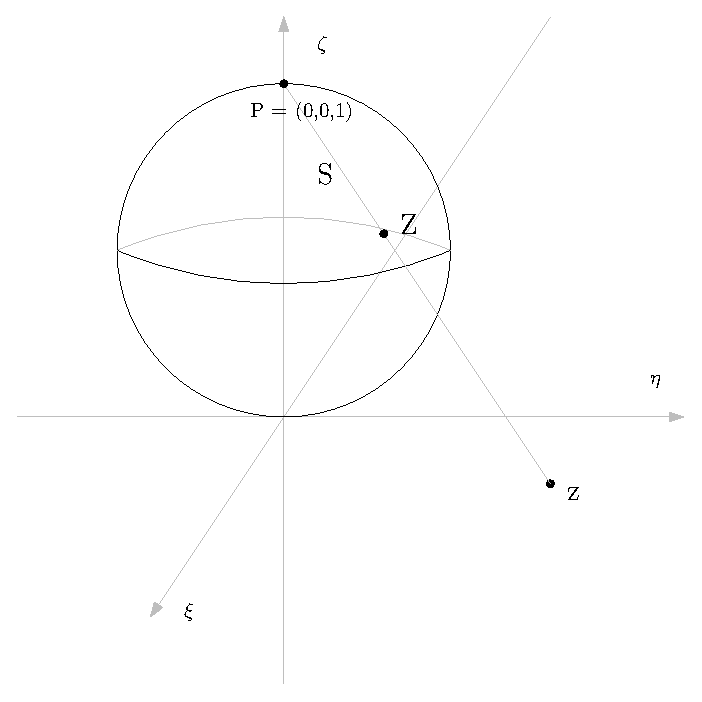
\includegraphics[scale=0.75]{Riemann.eps}
    \caption{Сфера Римана}
		\label{fig:2.1}
\end{figure}
\Def
\textbf{Стереографическая проекция:}
\begin{align*}
  & \forall z \in \CC \ \exists Z \in (\xi, \eta, \zeta): \ \left\{ \begin{matrix}
          \xi = tx \\
          \eta = ty \\
          \zeta = 1-t
      \end{matrix} \right., \ t \in [0;1]
\end{align*}
\begin{align*}
  & t = \frac{1}{1+ \left| z \right|^2}, \ \xi = \frac{x}{1+ \left| z \right|^2}, \ \eta = \frac{y}{1+ \left| z \right|^2}, \ \zeta = \frac{\left| z \right|^2}{1+ \left| z \right|^2}
\end{align*}
\begin{align*}
  & S \setminus P \leftrightarrow \CC, \ P \leftrightarrow \infty
\end{align*}
\textbf{Свойства}
\begin{enumerate}
    \item Любая пряая или окружность на комплексной плоскости переходит в
    окружность на сфере Римана.
    \item Если любые две кусочно гладкие кривые $\gamma_1$ и $\gamma_2$
    пересекаются под углом $\alpha$ на комплексной плоскости, то их образы
    $\tilde{\gamma}_1$, $\tilde{\gamma}_2$ будут пересекаться под тем же углом
    $\alpha$ на сфере Римана.
\end{enumerate}
\Def
$f: G \mapsto D$, где $G$~--- область, $D \subseteq \CCC$~--- область или вся
(расширенная) комплексная плоскость; $f(z) = u(x,y) + iv(x,y)$~---
\textbf{функция комплексного переменного.}
\Def
Пусть $z_0$~--- предельная точка $G \subseteq \CCC$ и $f: G \mapsto \CCC$; тогда
число $A$ назыается \textbf{пределом} $f$ в этой точке (пишется $\dst \lim_{z \to
  z_0} f(z_0)$) тогда и только тогда, когда выполняется
\begin{equation}\label{(2.3)}
    \forall \varepsilon > 0 \ \exists \delta(\varepsilon) > 0: \ z \in \os{\circ}{B}_\delta(z_0)\cap G \hookrightarrow f(z) \in B_\varepsilon (A)
\end{equation}
\asm
\begin{align*}
  & \exists \lim_{z \to z_0}f(z) = A = a+ib \Leftrightarrow \left\{ \begin{matrix}
          \dst \lim_{(x,y)\os{G}{\to}(x_0,y_0)}u(x,y) = a \\
          \dst \lim_{(x,y)\os{G}{\to}(x_0,y_0)}v(x,y) = b
      \end{matrix} \right.
\end{align*}
\pr
Очевидно по аналогии с последовательностями.
\Def
$f: G \mapsto \CCC$ \textbf{непрерывна} в $z_0 \in G \subseteq \CCC$, если
$z_0$~--- предельная точка $G$ и $\dst \lim_{z \to z_0} = f(z_0)$.
\asm
Функция непрерывна тогда и только тогда, кода ее действителная и мнимая части
непрерывны.
\pr Очевидно по аналогии с пределом.
\Def
\textbf{Функциональным рядом} называется сумма вида $\dst \sum_{n=1}^\infty
f_n(z)$, где $\forall n \in \NN \ f_n :G \mapsto \CC$.
\Def
Ряд \textbf{сходится равномерно}, если он:
\begin{enumerate}
    \item $\forall z \in G$ сходится к некоторой $S(z)$;
    \item $\forall \varepsilon > 0 \ \exists N(\varepsilon) > 0: \ \forall N \geq N
    (\varepsilon) \ \left| \dst \sum_{n=1}^Nf_n(z) - S(z) \right|\leq
    \varepsilon$.
\end{enumerate}
Все критерии и признаки для таких рядов аналогичны таковым в действительном
анализе.    
\newpage
\setcounter{section}{9}
\section{Глава 10. Кратные интегралы}
\subsection{Определение кратного интеграла}
\subsubsection{Случай, когда $f(x)$ - ограниченная функция.}
\begin{Def}
Пусть $f$ -- ограниченная функция, заданная на измеримом по Лебегу Жордану) множестве $E \subset \R^n$ конечной меры. 

$\textbf{Разбиением}$ множества $E$ называется $E=\bigsqcup\limits_{k=1}^N E_k$, где $E_k$ - измеримые по Лебегу (Жордану). \newline В качестве $\Delta x_k$ будем брать меру множеств $E_k$. 

Обозначим $M_k=\sup\limits_{x\in E_k} f\left(x\right) ,\  m_k=\inf\limits_{x\in E_k}f\left(x\right)$ \newline
Суммы Дарбу - Лебега (Жордана): верхняя $\mathcal{U}(P, f)=\sum\limits_{k=1}^N M_k \cdot \mu_{(J)}(E_k)$, нижняя $L(P, f)\?=\sum\limits_{k=1}^N m_k \cdot \mu_{(J)}(E_k)$.
\newline Верхний интеграл Лебега или Римана (L)(R)$\ \overline{I}_E(f)=\inf\limits_P \mathcal{U}(P, f)$,\newline Нижний интеграл Лебега или Римана (L)(R)$\ \underline{I}_E(f)=\sup\limits_P L(P, f)$
\end{Def}
\begin{Def}
Если (R)$\ \overline{I}_E(f)=$ (R)$\ \underline{I}_E(f)$, то $f$ называется интегрируемой по Риману на $E$, $\int\limits_E f(x)dx=$ (R)$\ \overline{I}_E(f)$ \newline
Если (L)$\ \overline{I}_E(f)=$ (L)$\ \underline{I}_E(f)$, то $f$ называется интегрируемой по Лебегу на $E$, $\int\limits_E f(x)d\mu (x)\?= \text{(L) }\overline{I}_E(f)$
\end{Def}
\textbf{Утв. 1} Функция $f$ интегрируема по Риману на $[a,b]$(в смысле старого определения) $\Leftrightarrow$ $f$ интегрируема по Риману на $E=[a,b] \subset \R^1$.
\begin{proof}
$(\Rightarrow)$	Составим цепочку неравенств:
\begin{equation}
\underline{I}(f) \overset{(1)}{\leqslant} \text{(R) }\underline{I}_{[a,b]}(f)\overset{(2)}{\leqslant} \text{(L) }\underline{I}_{[a,b]}(f)\overset{(3)}{\leqslant}\text{(L) } \overline{I}_{[a,b]}(f) \overset{(4)}{\leqslant} \text{(R) } \overline{I}_{[a,b]}(f)\overset{(5)}{\leqslant} \overline{I}(f)\tag{10.1.1}\label{10.1.1} 
\end{equation}

Неравенство (1) следует из того, что в старом определении мы делили на отрезки, которые пересекаются в концах, а в новом определении идет разбиение на непересекающиеся, измеримые по Жордану множества.

Неравенство (2) следует из того, что нижние интегралы в смысле Римана и в смысле Лебега отличаются тем, на какие множества мы разбиваем: измеримые по Жордану или Лебегу. Но так как каждое измеримое по Жордану автоматически измеримо по Лебегу, то в $\text{(L) }\underline{I}_{[a,b]}(f)$ мы берем точную верхнюю грань по большему множеству.

Неравенства (4), (5) следуют из выше доказанных, но в обратном порядке.

Доказательство неравенства (3): хотим установить, что для любых двух разбиений $P_1, P_2\ L(P_1, f) \leqslant \mathcal{U}(P_2, f)$, что и докажет требуемое неравенство. Для этого необходимо взять общее измельчение разбиений $P=P_1 \bigcup P_2$ и получить цепочку неравенств $L(P_1, f) \leqslant L(P, f) \leqslant \mathcal{U}(P, f) \leqslant \mathcal{U}(P_2, f)$. Получим это: составим два произвольных разбиения 
$P_1 : E = \bigsqcup\limits_{k=1}^{N_1} E_k^{(1)},\ P_2 : E = \bigsqcup\limits_{k=1}^{N_2} E_k^{(2)}$. Тогда общее измельчение $ P : E = \bigsqcup\limits_{k=1}^{N_1} \bigsqcup\limits_{j=1}^{N_2} E_k^{(1)} \bigcap E_j^{(2)}$.
Докажем неравенство для нижних сумм:

 $L(P_1, f)=\sum\limits_{k=1}^{N_1} \inf\limits_{x\in E_k^{(1)}}f(x) \cdot \mu_{(J)}(E_k^{(1)}) =
\sum\limits_{k=1}^{N_1} \inf\limits_{x\in E_k^{(1)}}f(x) \sum\limits_{j=1}^{N_2} \mu_{(J)} (E_k^{(1)}\bigcap E_j^{(2)})\?\leqslant \sum\limits_{k=1}^{N_1}\sum\limits_{j=1}^{N_2}\inf\limits_{x\in E_k^{(1)}\bigcap (E_j^{(2)}}f(x)\cdot \mu_{(J)} (E_k^{(1)}\bigcap E_j^{(2)})=L(P,f)$, так как инфимум по $E_k^{(1)}$ не превосходит инфимум по $E_k^{(1)}\bigcap E_j^{(2)}$ для каждого $j$. Аналогично доказывается оставшаяся часть неравенства.

Из доказанного неравенства \ref{10.1.1} следует, что из интегрируемости по Риману в старом смысле, мы получили интегрируемость в новом смысле, так как $\underline{I}(f) = \overline{I}(f)$, а также, что из интегрируемости по Риману следует интегрируемость по Лебегу.

$(\Leftarrow$)
Отступление.
Вспомним критерий интегрируемости:
$$f\in R[a,b] \Leftrightarrow (\forall \varepsilon > 0)(\exists P)\ \mathcal{U}(P, f)-L(P, f)<\varepsilon$$
В доказательстве мы использовали тот факт, что $\overline{I}(f)=\inf\limits_P \mathcal{U}(P, f)$, $\ \underline{I}(f)=\sup\limits_P L(P, f)$, и так как $\mathcal{U}(P, f)-L(P, f)<\varepsilon$, то и $\overline{I}(f) - \underline{I}(f) < \varepsilon$. Эта разность всегда неотрицательная, меньше любого положительного числа, значит равна 0. Вместо интегрируемости по Риману на отрезке можем написать интегрируемость по Риману на любом измеримом по Жордану или Лебегу.

Вернемся к доказательству.

 Пусть функция интегрируема по Риману в новом смысле: $\exists \int\limits_{[a,b]}f(x)dx$, тогда по критерию интегрируемости: $(\forall \varepsilon > 0)(\exists P:[a,b]=\bigsqcup\limits_{k=1}^{N} E_k) \mathcal{U}(P,f)-L(P,f)<\varepsilon$, где $E_k$ - измеримые по Жордану множества. Внутренняя мера Жордана $\mu_{*}^J(E_k)=\sup\limits_{M \subset E_k} |M|$, где $M$ - элементарное множество. Элементарным множеством на прямой является объединение конечного числа промежутков. Тогда 
$$\exists\text{ набор точек } \{a_j^{(k)}, b_j^{(k)}\},\ \bigsqcup\limits_{j=1}^{n_k}[a_j^{(k)}, b_j^{(k)}] \subset E_k,\ \mu_jE_k \backslash \bigsqcup \limits_{j=1}^{n_k}[a_j^{(k)}, b_j^{(k)}]) < \dfrac{\varepsilon}{2\cdot C \cdot N},$$
\mbox{где $|f(x)|\leqslant C$. Возьмем разбиение в старом смысле $Q: a=x_0 < x_1 < \ldots < x_{\nu} = b,$} $\text{где множество точек }\{x_i\}_{i=1}^{\nu} = \{a_j^{(k)}, b_j^{(k)}\}_{j=1}^{n_k},  k=\overline{1,\ldots,N}$.
Оценим $\mathcal{U}(Q, f)-L(Q, f)=\sum\limits_{i=1}^{\nu}(\sup\limits_{[x_{i-1}, x_i]}f(x)-\inf\limits_{[x_{i-1}, x_i]}f(x))\cdot \Delta x_i = \sum\limits_{k=1}^N \sum\limits_{j=1}^{n_k}(\sup\limits_{x\in [a_j^{(k)},b_j^{(k)}]}f(x)-\inf\limits_{x\in [a_j^{(k)},b_j^{(k)}]}f(x) )(b_j-a_j )+\sum\limits_{x\in B}(\sup\limits_{[x_{i-1}, x_i]}f(x)-\inf\limits_{[x_{i-1}, x_i]}f(x))\Delta x_i \leqslant \sum\limits_{k=1}^N(M_k-m_k)\sum\limits_{j=1}^{n_k}(b_j-a_j)+\sum\limits_{i\in B}\ldots \leqslant \sum\limits_{k=1}^N (M_k-m_k)\cdot \mu_{J}(E_k)+2\cdot C\cdot \sum\limits_{i\in B}\Delta x_i < 2\varepsilon$
\end{proof}
.
\begin{wrapfigure}{r}{0.5\linewidth}
	\includegraphics[width=\linewidth]{images/1.png}
\end{wrapfigure}
\begin{Def}
	\mbox{Пусть $ f:E\to\mathbb{R} $} ---  ограниченная измеримая на измеримом по Лебегу множестве \mbox{$ E\subset\mathbb{R}^n $} конечной меры функция.

	Если $ M=\sup\limits_{x\in E}f(x), $ $ m=\inf\limits_{x\in E}f(x), $ то \textbf{разбиением Лебега}, отвечающим разбиению $ Q=\{m=y_0<y_1<\ldots <y_N=M\}, $ называется разбиение
	$ P: E=\bigsqcup\limits_{i=1}^{N}E_i$, \mbox{где $E_i=\{x\in E: fx)\in [y_{i-1}, y_i)\},$} $i=1, \ldots, N-1$.
	\newline
	$E_N= \{x\in E: fx)\in [y_{N-1}, y_N]\}$
	\newline
	\newline
	\mbox{Тогда интегральной суммой Лебега назовем $S(Q, f, \{t_i\})=\sum\limits_{i=1}^N f(t_i)\mu(E_i)$, где $t_i \in E_i,$}$ 
	\newline i = 1, \ldots, N$.
\end{Def} 
\begin{theorem}(Основная теорема об интеграле Лебега от ограниченных функций).
	Если $f(x)$ ограниченная измеримая на измеримом по Лебегу множестве $ E\subset\R^n $ конечной меры  функция, то она интегрируема по Лебегу (суммируема) на $E$, причем ее интеграл равен пределу интегральных сумм с разбиениями Лебега, отвечающими разбиениям  $ Q $, при стремящемся к нулю диаметре последнего, т.е. $$\int\limits_E f(x)d\mu(x)=\lim_{\Delta(Q)\to 0}S(Q,f,\{t_i\}).$$
	Это значит, что $(\forall \varepsilon >0)(\exists \delta > 0)(\forall Q, \Delta(Q)<\delta) \text{ и } \forall \{t_i\}, t_i \in E_i, i=1,\ldots, N,$ где $E=\bigsqcup\limits_{i=1}^N E_i$ --- разбиение Лебега, отвечающее разбиению $Q$ отрезка $[m, M]$, выполняется $|S(Q, f, \{t_i\})-\int\limits_E f(x)d\mu(x)|<\varepsilon$.
\end{theorem}

\begin{proof}
	Прежде всего заметим, что если $P: E=\bigsqcup\limits_{i=1}^N E_i$, то\newline $L(P, f)\leqslant S(Q, f, \{t_i\})\leqslant \mathcal{U}(P, f)$. Кроме того $\mathcal{U}(P, f) - L(P, f) = \sum\limits_{i=1}^N(M_i-m_i)\mu(E_i) \?\leqslant \sum\limits_{i=1}^N (y_i-y_{i-1})\cdot\mu(E_i)\leqslant \Delta(Q) \sum\limits_{i=1}^N\mu(E_i)=\Delta(Q)\mu(E)$. В качестве $\delta = \dfrac{\varepsilon}{\mu(E)}$. Для множеств $ E $ меры нуль утверждение очевидно, так как все суммы (верхние, нижние, интегральные) в этом случае равны нулю.
\end{proof}

\subsubsection{Случай, когда $f(x)\geqslant 0$.}
Пусть $f(x)\geqslant 0$ - измеримая на измеримом по Лебегу множестве $E$ конечной меры функция. В качестве разбиений будем допускать и разбиения на счетное число измеримых по Лебегу множеств: $E = \bigsqcup\limits_{i=0 }^{\infty}E_i,\ E_0:=\{x\in E:f(x)=+\infty\}$. Обратите внимание! Индексацию ведем с 0, и $E_0$ жестко фиксируем. Соглашение: если $\mu(E_0)=0$, то $(+\infty)\cdot \mu(E_0)=0$. Получаем, что мы ничего не можем сказать о $M$, а $m=0$. 

Тогда разбиение принимает вид $Q: 0=y_0<y_1<\ldots$. 

В качестве $E_i = \{x\in E: f(x)\in[y_{i-1}, y_i)\}, i=1,\ldots$.

$\Delta(Q):=\sup\limits_{i=1, \ldots}(y_i-y_{i-1})$, может равняться и $+\infty$.

$L(P, f)=\sum\limits_{i=0}^{\infty}m_i\cdot \mu(E_i),\  \mathcal{U}(P, f)=\sum\limits_{i=0}^{\infty}M_i\cdot \mu(E_i)$ 

\begin{theorem}Основная теорема об интеграле Лебега для неограниченных измеримых функций)
Если $f(x)$ - неотрицательная, измеримая на измеримом по Лебегу множестве $E\subset \R^n$ конечной меры, то она интегрируема по Лебегу на $E$, причем
$\int\limits_E f(x)d\mu(x)\?=\lim\limits_{\Delta(Q)\to0}S(Q, f, \{t_i\}).$ 

При конечном значении интеграла понятие предела такого вида -- то же, что и в предыдущей основной теореме, если же интеграл бесконечен, то требуется, чтобы \newline$(\forall \varepsilon>0)( \exists \delta > 0)(\forall Q, \Delta(Q)<\delta) \text{ и } \forall \{t_i\}, t_i \in E_i, i=1,\ldots$, где $E=\bigsqcup\limits_{i=1}^{\infty} E_i$ --- разбиение Лебега, отвечающее разбиению $Q$ полуоси $[0, +\infty)$, выполняется $S(Q, f, \{t_i\})\geqslant\varepsilon$.
\end{theorem}

\begin{proof}
В случае конечного интеграла, доказательство аналогично доказательству предыдущей теоремы. Если интеграл бесконечен, то и предел интегральных сумм бесконечность, так как все $S$ зажаты между $\mathcal{U}(P, f) \:\text{и} \:L(P, f)$.
\end{proof}

\begin{Def}
Если $\int\limits_E f(x)d\mu(x) < +\infty$, то $f$ называется суммируемой на $E$.
\end{Def}

\subsubsection{Случай, когда $f(x)$ - любого знака.}
Пусть $f(x)$ измерима на измеримом по Лебегу множестве $E \subset \R^n$ конечной меры. Введем $f_+(x):=\max(f(x), 0), f_-(x):=\max(-f(x), 0)$ - это неотрицательные, измеримые функции. Такие функции интегрируемы по Лебегу, то есть существуют $\int\limits_E f_+(x)d\mu(x), \int\limits_E f_-(x)d\mu(x)$. Если хотя бы один из этих интегралов конечен, то $f$ называется интегрируемой по Лебегу. Если оба конечны, то $f$ - суммируемая на $E$.
$$\int\limits_E f_+(x)d\mu(x)- \int\limits_E f_-(x)d\mu(x) = \int\limits_E f(x)d\mu(x)$$
Пример измеримой, но не интегрируемой по Лебегу функции: возьмем отрезок, на одной его половине функция равна $+\infty$, на другой $-\infty$.



\newpage
\section{Лекция 3. Недетерминированные конечные автоматы.}

Вспомним формальное определение (\ref{eq:FA}) конечного автомата.

\textbf{\text{Конечный автомат }} $\mathcal{A}$ --- устройство, описываемое набором $\langle Q$, $\Sigma$, $q_0$, $\delta$, $F \rangle$:
\begin{enumerate}
  \item {\bfseries\itshape{Q}} - конечное множество состояний автомата;
  \item $\boldsymbol{\Sigma}$ - алфавит, слова над которым обрабатывает автомат;
  \item $\boldsymbol{q_0}$ - начальное состояние автомата;
  \item $\boldsymbol{\delta}$ : $Q \times (\Sigma\cup\{\varepsilon\} ) \rightarrow 2^{Q}$ - функция переходов
  \item $\boldsymbol{F} \subset \boldsymbol{Q}$ - множество принимающих состояний.
\end{enumerate}


\begin{wrapfigure}{r}{0.3\textwidth}
  \centering
  \begin{tikzpicture}[node distance=2cm,on grid,auto]
    \node[state,initial] (q_0)   {$q_0$};
    \node[state,accepting] (q_1) [right=of q_0] {$q_1$};
    \path[->]
    (q_0) edge [bend left] node {$b$} (q_1)
    (q_0) edge [loop above] node {$a,b$} ()
    (q_1) edge [bend left] node {$\varepsilon$} (q_0);
  \end{tikzpicture}
  \caption{Пример НДА.}
  \label{fig:NFAexample}
\end{wrapfigure}

Рассмотрим рисунок (\ref{fig:NFAexample}). К примеру сразу из определения и графа имеем: $\delta(q_0,\:b)=\{q_0,q_1\}$.

\begin{question}
  Неформально опишите язык, распознаваемый данным автоматом.
\end{question}

\begin{nonum}
  Язык $R$, состоящий из слов, оканчивающихся на $b$.

  В самом деле, в принимающее состояние можно перейти по единственному переходу на котором написан символ $b$, то есть $L(\mathcal{A})\subseteq R$.
  Далее любое слово, оканчивающееся на $b$ принимается автоматом, потому что, обрабатывая все символы слова автомат может оставаться в состояний
  $q_0$, а когда встретится последний символ(он же буква $b$) перейти в состояние $q_1$. Итак, $R\subseteq L(\mathcal{A})$.
\end{nonum}

\subsection{Алгоритм проверки принадлежности слова языку, распознаваемому НКА.} \label{alg:word}

В случае ДКА все тривиально. Просто эмулируем работу автомата на входном слове. Каждое следующее состояние определяется однозначно.
Обработав слово за линейное время выясняем принимается ли оно автоматом.

В случае НКА может быть несколько путей вычесления, к примеру для слова $bb$ в автомате на рисунке (\ref{fig:NFAexample})
есть более одного пути: $$q_0\xrightarrow{b} q_0\xrightarrow{b} q_1,$$
$$q_0\xrightarrow{b} q_1\xrightarrow{\varepsilon} q_0\xrightarrow{b} q_0.$$

Заметим, что не обязательно все возможные пути заканчиваются в принимающем(или не принимающем) состоянии, в приведенном примере один путь
заканчивается, другой --- нет.

\paragraph*{Алгоритм.} Пусть есть слово $w = w_1w_2\ldots w_n$, $w_i\in\Sigma^*$. На $i$"=ом шаге будем помнить и пересчитывать множество состояний
$Q_i=\{q\:|\:q_0\xrightarrow{w[1,i]}q\}$.

Итак, если после обработки слова, в $Q_n$ есть принимающее состояние, то слово принимается.
Для более формального описания алгоритма, введем функцию
$$\varepsilon\text{-closure}(S)=S\cup \{q\:|\:\exists p\in S\: :\: p\xrightarrow{\varepsilon}q\}$$

Наконец, опишем алгоритм формально:

\begin{enumerate}
  \item Построить множество $Q_0$ = $\varepsilon$"=closure($q_0$).
  \item Для $k$ от 1 до $|w|$ построить множества:
        \begin{itemize}
          \item $Q_k'=\{p\:|\:\exists q\in Q_k\: :\: p\in\delta(q,\:w_k)\}$;
          \item $Q_{k+1}=\varepsilon\text{-closure}(Q_k')=\displaystyle{\bigcup _{q'\in Q_k'}}\varepsilon\text{-closure}(q')$;
        \end{itemize}
  \item Если $Q_{|w|}\cap F_{\mathcal{A}}\neq \varnothing$, то ответ <<Да>>, иначе <<Нет>>.
\end{enumerate}


\begin{question}
  Как эффективно вычислить $\varepsilon\text{-closure}(S)$?
\end{question}

\begin{nonum}
  Рассмотрим подграф графа автомата, в котором оставлены только ребра, на которых написано $\varepsilon$.
  И дальше для каждого состояния из $S$ обходом в глубину(или в ширину) будем искать все достижимые состояния.
\end{nonum}


\subsection{Построение НКА по РВ.}

Напомним, что по определению любой регулярный язык
можно построить согласно следующей схеме:

\begin{enumerate}
  \item $\varnothing \in REG$
  \item $\forall\sigma \in \sum \implies \{\sigma\} \in  REG$
  \item $\forall X, Y \in REG: X \circ Y, X|Y, X^* \in REG$
\end{enumerate}

Мы будем строить НКА по РВ для каждого пункта. Более того,
нам потребуется соблюсти технические условия:

\begin{enumerate}[(i)]
  \item НКА имеет ровно одно принимающее состояние;
  \item В начальное состояние НКА не ведёт ни один переход;
  \item Из принимающего состояния НКА нет ни одного перехода.
\end{enumerate}

\begin{question}
  Построить такой автомат для
  \begin{itemize}
    \item Пустого языка;
    \item Языка, состоящего из одного символа.
  \end{itemize}
\end{question}


\begin{nonum}
  Приведем только ответы, корректность очевидна.

  \begin{figure}[!h]
    \centering
    \begin{minipage}{.5\textwidth}
      \centering
      \begin{tikzpicture}[node distance=2cm,on grid,auto]
        \node[state,initial] (q_0)   {$q_0$};
        \node[state,accepting] (q_1) [right=of q_0] {$q_1$};
      \end{tikzpicture}
      \caption{Пустой язык.}
    \end{minipage}%
    \begin{minipage}{.5\textwidth}
      \centering
      \begin{tikzpicture}[node distance=2cm,on grid,auto]
        \node[state,initial] (q_0)   {$q_0$};
        \node[state,accepting] (q_1) [right=of q_0] {$q_1$};
        \path[->]
        (q_0) edge node {$a$} (q_1);
      \end{tikzpicture}
      \caption{Язык $\{a\}$.}
    \end{minipage}
  \end{figure}
\end{nonum}


Осталось построить автоматы для пункта (3) определения регулярного языка. Будем изображать НКА схематично, помечая в них только начальное и принимающее состояния:
\begin{figure}[!h]
  \centering
  \begin{tikzpicture}[node distance=2cm,on grid,auto]
    \draw (0.5,0) ellipse (3cm and 1.5cm);
    \node[state,initial] (q_0)   {$q_0$};
    \node[] at (1,0) {$\mathcal{A}$};
    \node[state,accepting] (q_1) [right=of q_0] {$q_1$};
  \end{tikzpicture}
  \caption{Автомат, удовлетворяющий условиям (i–iii).}
\end{figure}

Далее, мы будем предполагать, что начальное состояние на схеме
находится слева, а принимающее справа.
Допустим уже построены автоматы $\mathcal{A}$ и $\mathcal{B}$ (удовлетворяющие условиям (i–iii)) для регулярных языков
$X$ и $Y$ соответственно. Построим
явно автомат, распознающий $X \cdot Y$.

\begin{figure}[!ht]
  \centering
  \begin{tikzpicture}[node distance=4.5cm,on grid,auto,initial text=]
    \draw (1,0) ellipse (2cm and 1cm);
    \draw (3.5,0) ellipse (2cm and 1cm);
    \draw (2.25, 0) circle (0.5cm);
    \node[state,initial] (q_0)   {$q_0^{\mathcal{A}}$};
    \node[state,accepting] (q_1) [right=of q_0] {$q_F^{\mathcal{B}}$};
    \node[] at (1,0) {$\mathcal{A}$};
    \node[] at (3.5,0) {$\mathcal{B}$};
  \end{tikzpicture}
  \caption{Автомат для конкатенации.}
  \label{fig:concatFA}
\end{figure}

Как видно из рисунка \ref{fig:concatFA}, результирующий автомат получен из автоматов $\mathcal{A}$ и $\mathcal{B}$
следующим образом. Начальное состояние автомата $\mathcal{B}$
\textit{склеено} с начальным состоянием автомата $\mathcal{A}$:
мы удалили из автомата $\mathcal{B}$ начальное состояние $q_0^{\mathcal{B}}$, а все переходы, которые вели из него,
добавили к принимающему состоянию $q_F^{\mathcal{A}}$
автомата $\mathcal{A}$, которое сделали непринимающим.
Дабы определить склейку состояний для произвольных автоматов, скажем, что если бы в состояние $q_0^{\mathcal{B}}$ вели какие-то
переходы, то их бы также направили в состояние, полученное в результате склейки.


Далее строим автомат для языка $X | Y$ используя конструкцию:

\begin{figure}[!ht]
  \centering
  \begin{tikzpicture}[node distance=3cm,on grid,auto,initial text=]
    \node[state,initial] (q_0)   {$q_0$};
    \node[state] (q_0a) [above right=of q_0] {$q_0^{\mathcal{A}}$};
    \node[state] (q_fa) [right=of q_0a] {$q_F^{\mathcal{A}}$};
    \node[state] (q_f) [below right=of q_fa] {$q_F$};
    \node[state] (q_0b) [below right=of q_0] {$q_0^{\mathcal{B}}$};
    \node[state] (q_fb) [right=of q_0b] {$q_F^{\mathcal{B}}$};
    \node[] at (3.6, 2.1) {$\mathcal{A}$};
    \node[] at (3.6, -2.1) {$\mathcal{B}$};
    \draw (3.6, 2.1) ellipse (2.5cm and 1cm);
    \draw (3.6, -2.1) ellipse (2.5cm and 1cm);
    \path[->]
    (q_0) edge node {$\varepsilon$} (q_0a)
    (q_0) edge node {$\varepsilon$} (q_0b)
    (q_fa) edge node {$\varepsilon$} (q_f)
    (q_fb) edge node {$\varepsilon$} (q_f);
  \end{tikzpicture}
  \caption{Автомат для конкатенации.}
  \label{fig:sumFA}
\end{figure}


И наконец перейдём к построению автомата для языка $X^*$:


\begin{figure}[!ht]
  \centering
  \begin{tikzpicture}[node distance=2.5cm,on grid,auto,initial text=]
    \node[state,initial] (q_0)   {$q_0$};
    \node[state] (q_0a) [right=of q_0] {$q_0^{\mathcal{A}}$};
    \node[state] (q_fa) [right=of q_0a] {$q_F^{\mathcal{A}}$};
    \node[state] (q_f) [right=of q_fa] {$q_F$};
    \draw (3.75,0) ellipse (2cm and 1cm);
    \node[] at (3.75,-0.5) {$\mathcal{A}$};
    \path[->]
    (q_0) edge node {$\varepsilon$} (q_0a)
    (q_0) edge [bend left] node {$\varepsilon$} (q_f)
    (q_fa) edge [bend right] node {$\varepsilon$} (q_0a)
    (q_fa) edge node {$\varepsilon$} (q_f);
  \end{tikzpicture}
  \caption{Автомат $C$ для итерации.}
  \label{fig:iterFA}
\end{figure}


\begin{proof}

  По индукции докажем, что для $\forall n>0$ $w\in X^n\Rightarrow w\in L(C)$, то есть докажем включение $X^*\subseteq L(C)$.

  \underline{База}: пустое слово принимается автоматом.

  \underline{Переход}: Рассмотрим слово $w=u_1\cdot u_2\cdot\ldots\cdot u_n$, $u_i\in L(\mathcal{A})$. Слово
  $v=u_1\cdot u_2\cdot\ldots\cdot u_{n-1}\in L(C)$ по предположению индукции. Есть несколько вариантов.
  \begin{itemize}
    \item $v$ --- пустое. Но тогда можно попасть в состояние $q_0^{\mathcal{A}}$, а из него, так как $u_n$ принимается $\mathcal{A}$,
          в состояние $q_F^{\mathcal{A}}$, откуда уже в $q_F$.
    \item $v$ --- непустое. Это означает, что путь по нему из начального состояния в принимающее обязательно прошел через
          $q_F^{\mathcal{A}}$. Тогда вернемся на шаг назад в состояние $q_F^{\mathcal{A}}$, а из него еще на шаг в состояние
          $q_0^{\mathcal{A}}$ по ребру $\varepsilon$. И оттуда уже обрабатываем слово $u_n$.
  \end{itemize}

  Теперь докажем $L(C)\subseteq X^*$.

  Пусть слово $w\in L(c)$. Если $w$ --- пустое, то оно очевидно принадлежит $X^*$. Если же слово не пустое, посмотрим на путь из $q_0$.
  Если этот путь не проходил через ребро $q_F^{\mathcal{A}}\xrightarrow{\varepsilon} q_0^{\mathcal{A}}$, тогда все очевидно.

  Если же этот переход был, найдем первый этот переход, который случился после того, как был обработан какой-то непустой префикс слова $w$.
  Заметим, что этот префикс есть собственный префикс $w$ и по предположению индукции этот префикс принадлежит $X^*$. Заметим, что и суффикс принадлежит
  $X^*$, но тогда и $w$ принадлежит $X^*$.

\end{proof}


\subsection{Построение ДКА по НКА.}

Модифицируем алгоритм проверки принадлежности слова языку, распознаваемому НКА. Заметим, что число множеств $Q_k$,
появлявшихся в алгоритме, конечно, поскольку $Q_k \subseteq 2^{Q_{\mathcal{A}}}$. Поэтому всевозможные множества
можно хранить в конечной памяти, они и будут состояниями ДКА, который мы назовём $2^{\mathcal{A}}$.
Начальным состоянием будет состояние $Q_0$,
принимающими будут множества $Q_k$, содержащие принимающие состояния $\mathcal{A}$, а переходы между состояниями определены, как и в алгоритме:

\begin{enumerate}
  \item $Q_0 = \varepsilon\text{-closure}(q_0)$
  \item $\delta (Q', a)=\varepsilon\text{-closure}(\widetilde{Q}')$, где
        $\widetilde{Q}'=\{q\:|\: \exists p\in Q':\:p\in\delta(p, a)\}=\displaystyle{\bigcup_{p\in Q'}}\delta(p, a).$
\end{enumerate}


\subsection{Построение РВ по НКА.}

\begin{Def}
  \textit{Обобщенный НКА} --- НКА, у которого вместо букв на переходах написаны регулярные выражения.

  Слово $w\in L(\mathcal{A})$, если существует разбиение $w=u_1\cdot u_2\cdot\ldots\cdot u_n$, $u_i\in \Sigma^*$ и существует
  последовательность состояний $q_1, q_2, \ldots, q_n\in F$, такие что $u_1\in R_{q_0, q_1}$, $u_2\in R_{q_1, q_2}$, \ldots, $u_n\in R_{q_{n-1}, q_n}$, где
  $R_{q_i,q_j}$ --- РВ написанное на ребре $q_i\rightarrow q_j$.
\end{Def}

Основная идея такая. Вначале нужно превратить НКА в НКА с одним принимающем состоянием, в который не ведет ни одно ребро и с начальным состоянием
в которое также ничего не ведет (рисунок (\ref{fig:prepare})).

\begin{figure}
  \centering
  \begin{tikzpicture}[node distance=3cm,on grid,auto,initial text=]
    \node[state,initial] (q0)   {$q_0$};
    \node[state, initial] (q1) at (1,3) {};
    \node[state,accepting] (p) at (5, 0) {$p$};
    \node[state,accepting] (r1) at (4.5, 2.5) {};
    \node[state,accepting] (r2) at (3, 2) {};
    \node[state,accepting] (r3) at (5, 4) {};
    \draw (3,3) ellipse (4cm and 2cm);
    \path[->]
    (q0) edge node {$\varepsilon$} (q1)
    (r1) edge node {$\varepsilon$} (p)
    (r2) edge node {$\varepsilon$} (p)
    (r3) edge [bend left, out=30, in=120] node {$\varepsilon$} (p);
  \end{tikzpicture}
  \caption{Начальная подготовка графа.}
  \label{fig:prepare}
\end{figure}


Далее делаем старые принимающие состояние непринимающими и переходим к следующему шагу.

Берем НКА и последовательно удаляем состояния, пересчитывая ребра.

\begin{wrapfigure}{r}{0.45\textwidth}
  \centering
  \begin{tikzpicture}[node distance=2.5cm,on grid,auto,initial text=]
    \node[state,initial] (q)   {$q$};
    \node[state] (p) [right=of q] {$p$};
    \node[state] (r) [right=of p] {$r$};
    \path[->]
    (q) edge node {$R_{q,p}$} (p)
    (p) edge node {$R_{p,r}$} (r)
    (p) edge [loop above] node {$R_{p,p}$} ()
    (q) edge [bend right, in=240] node {$R_{q,r}$} (r);
  \end{tikzpicture}
  \caption{Удаление состояния.}
  \label{fig:deleteNode}
\end{wrapfigure}


Допустим нужно удалить состояние $p$. Нужно рассмотреть все пары $(q, r)$ удовлетворяющие
рисунку (\ref{fig:deleteNode}).
Тогда после удаления $p$ нужно убрать все ребра на рисунке и добавить ребро $q\xrightarrow{R'_{q, r}}r$, где $$R'_{q,r}=R_{q,r}\cup R_{q,p}R^*_{p,p}R_{p,r}$$.

\newpage
\begin{flushright}
    \textit{Лекция 4 (от 15.09)}
\end{flushright}

\textbf{Кривая} $\gamma$~--- класс эквивалентных параметризаций $z(t) = x(t) +
iy(t), \ t \in \left[ t_0; t_1 \right]$
\\
\textbf{Параметризации эквивалентны}, если существует монотонная возрастающая
функция $\psi(\tau) = t$, сохраняющая направление.
\\
\textbf{Гладкая кривая (ГК)}~--- такая кривая $\gamma$, что существует параметризация
$z(t) = x(t) + iy(t)$, $x \in C^1 \left( \left[ t_0; t_1 \right] \right)$, $y
\in C^1 \left( \left[ t_0; t_1 \right] \right)$, $\forall t \in \left[ t_0; t_1
\right] \ z'(t) \neq 0$.
\\
\textbf{Замкнутая ГК (ЗГК)}~--- такая ГК, что $z(t_0) = z(t_1)$, $z'(t_0+0) =
z'(t_1-0)$.
\\
\textbf{Кусочно гладкая кривая (КГК)}~--- такая непрерывная кривая $\gamma$, что
$\exists t_0 = \theta_0 < \theta_1 < \dots < \theta_{n-1} < \theta_n = t_1$, что
$\forall k \ \gamma_k: \ z(t), \ t \in [\theta_{k-1}, \theta_k]$ есть ГК.
\\
\textbf{Разбиение} отрезка $\left[ t_0, t_1 \right]$: $\lambda = \{t_0 = \tau_0
< \tau_1 < \dots < \tau_{m_\lambda} = t_1\}$.
\\
\textbf{Мелкость (диаметр)} разбиения $\lambda$ $\left| \lambda \right| = \dst
\max_{k \{1, \dots, m_\lambda\}}\left| \tau_k - \tau_{k-1} \right|$.
\Def Пусть $f: \gamma \mapsto \CC$ непрерывна на КГК $\gamma$. Пусть
$\lambda$~--- разбиение $\left[ t_0, t_1 \right]$ для $\gamma: \ z(t)$~---
кусочно гладкой. Пусть $z(t_k) = z_k, \ k \in \{0, \dots, m_\lambda\}$, $\zeta_k
\in \gamma_k = \gamma_{z_{k-1}z_k}$
\begin{align*}
  & \sigma(\lambda) = \sum_{k = 1}^{m_{\lambda}} f(\zeta_k) \Delta z_k
\end{align*}
$\Delta z_k = z_k - z_{k-1}$~--- \textbf{интегральная сумма};
\\
если $\exists \lim \sigma(\lambda) \ \forall \zeta_k, \ \left| \lambda \right|
\to 0$, то этот предел называется \textbf{интегралом Римана от $f$ по $\gamma$}
и записывается как
\begin{equation} \label{(6.1)}
    \int_{\gamma}f(z) dz
\end{equation}
\theorem
Если условия определения интеграла выполняются, то он существует и справедливо:
\begin{equation} \label{(6.2)}
    \int_{\gamma}f(z)dz = \int_{\gamma}\left( u dx - v dy \right) + i \int_\gamma \left( v dx + u dy \right)
\end{equation}
\pr
\begin{align*}
  & \sigma(\lambda) = \sum_{k = 1}^{m_\lambda}\left( u(\xi_k, \eta_k) + iv(\xi_k, \eta_k) \right)\left( \Delta x_k + i \Delta y_k \right) = \sum_{k = 1}^{m_\lambda}\left( u(\xi_k, \eta_k) \Delta x_k - v(\xi_k, \eta_k) \Delta y_k\right) + \\
  & + \left( v(\xi_k, \eta_k) \Delta x_k + u(x_k, y_k) \Delta y_k\right) = \sigma_1(\lambda) + \sigma_2(\lambda) \to \int_{\gamma}\left( u dx - v dy \right) + i \int_\gamma \left( v dx + u dy \right)
\end{align*}
\corollary
Если условия определения интеграла выполняются, то верно:
\begin{equation} \label{(6.3)}
    \int_\gamma f(z) dz = \int_{t_0}^{t_1}f(z(t))z'(t)dt
\end{equation}
\begin{equation} \label{(6.4)}
    \gamma: z(t), \ \int_{t_0}^{t_1}\left( P(t) + iQ(t) \right) dt = \int_{t_0}^{t_1}P(t)dt + i \int_{t_0}^{t_1}Q(t)dt
\end{equation}
\pr
Из \eqref{(6.2)} и свойств криволинейных интегралов II рода
\begin{align*}
  &\int_{\gamma}P(x,y) dx + Q(x,y)dy = \int_{t_0}^{t_1} \left( P(x(t), y(t))x'(t) + Q(x(t), y(t))y'(t) \right) dt
\end{align*}
\underline{\textbf{Общие свойства интеграла}}
\begin{enumerate}
    \item Линейность:
    \begin{align*}
      &\int_{\gamma}\left(\lambda f(z) + \mu g(z)\right) dz = \lambda\int_{\gamma}f(z) dz + \mu \int_\gamma g(z) dz
    \end{align*}
    \item Аддитивность вдоль кривой: если $\gamma = \gamma_1 \cup \gamma_2$
    (общая точка~--- только конец), то
    \begin{align*}
      &\int_{\gamma}f(z) dz = \int_{\gamma_1}f(z) dz + \int_{\gamma_2} f(z) dz
    \end{align*}
    \item Изменение знака при смене направления: если $\gamma^{-1}$~---
    кривая, совпадающая во всех точках с $\gamma$, но противоположно
    направленная, то
    \begin{align*}
      &\int_{\gamma^{-1}}f(z) dz = - \int_{\gamma}f(z) dz
    \end{align*}
    \item Инвариантность относительно замены параметра.
    \item Выполняется неравенство:
    \begin{equation} \label{(6.5)}
        \left| \int_\gamma f(z) dz \right| \leq \int_{\gamma}\left| f(z) \right| \cdot \left| dt \right| = \int_{t_0}^{t_1} \left| f(z(t)) \right| \sqrt{(x'(t))^2 + (y'(t))^2}dt
    \end{equation}
    \pr
    Из \eqref{(6.3)}:
    \begin{equation} \label{(6.6)}
        \left| \sigma(\lambda) \right| \leq \sum_{k = 1}^{m_\lambda}\left| f(\zeta) \right| \cdot \left| \Delta z_k \right|
    \end{equation}
\end{enumerate}
\example
\begin{align*}
  &J_k = \int_{\gamma: \left| z-a \right| = r} (z-a)^k dz, \ k \in \ZZ
\end{align*}
Параметр: $z(t)= a+re^{it}, \ t \in [0;2\pi]$
\begin{align*}
  & dz(t) = rie^{it}dt
\end{align*}
\begin{align*}
  &J_k = \int_{0}^{2\pi} r^ke^{ikt}rie^{it}dt = r^{k+1}i\int_{0}^{2\pi}e^{i(k+1)t} dt
\end{align*}
\begin{align*}
  &J_{-1} = 2 \pi i
\end{align*}
\begin{align*}
  &J_k = r^{k+1}i\int_{0}^{2\pi} \left( \cos(k+1)t + i \sin(k+1)t \right) dt = 0, \ k \neq -1
\end{align*}
\example
\begin{align*}
  &J_1 = \int_{\gamma} dz, \ J_2 = \int_{\gamma}z dz
\end{align*}
$\gamma: z(t)$, и согласно \eqref{(6.3)}
\begin{align*}
  &J_1 = \int_{t_0}^{t_1} z'(t)dt = z(t_1) - z(t_0)
\end{align*}
\begin{align*}
  &J_2 = \int_{t_0}^{t_1} z(t)z'(t)dt = \frac{1}{2}\int_{t_0}^{t_1}\frac{d}{dt}\left( z^2(t) \right)dt = \frac{1}{2}\left( z^2(t_1) - z^2(t_0) \right)
\end{align*}
\theorem
Пусть $f_n: G \mapsto \CC$ непрерывна на $G$ $\forall n \in \NN$, $\gamma$~---
КГК, $\gamma \subseteq G$.
\\
Пусть $\dst \sum_{n=1}^{\infty}f_n(z) \underset{\gamma}{\rightrightarrows} S(z)
\ \forall z \in \gamma$.
Тогда $S(z)$ непрерывна на $\gamma$ и выполняется
\begin{equation} \label{(6.7)}
    \int_{\gamma}S(z) dz = \sum_{n=1}^{\infty}\int_{\gamma}f_n(z)dz
\end{equation}
\pr
Ряд сходится равномерно на $\gamma$
\begin{align*}
  & \Updownarrow
\end{align*}
\begin{equation} \label{(6.8)}
    \forall \varepsilon > 0 \ \exists N(\varepsilon): \ \forall N\geq N(\varepsilon) \ \underset{z \in \gamma}{\sup} \left| S(z) - \sum_{n = 1}^{N}f_n(z) \right| = \underset{z \in \gamma}{\sup} \abs{S - S_N(z)} \leq \varepsilon
\end{equation}
\begin{align*}
  &\exists \delta > 0: \ \forall z_0 \in \gamma, \ z \in \gamma, \ \left| z - z_0 \right| < \delta: \ \left| S(z) - S(z_0) \right| \leq \left| S(z) - S_N(z) \right| +  \left| S_N(z) - \right. \\
  &\left. - S_N(z_0) \right| + \left| S_N(z_0) - S(z_0) \right| \leq \left| S_N(z) - S_N(z_0) \right| + 2 \varepsilon \leq 3 \varepsilon
\end{align*}
\begin{align*}
  & \Downarrow
\end{align*}
\begin{align*}
  & S(z) \rightarrow S(z_0)
\end{align*}
\begin{align*}
  & \Downarrow
\end{align*}
\begin{align*}
  & \exists \int_{\gamma}S(z)dz
\end{align*}
\begin{align*}
  &\forall N \geq N(\varepsilon) \ \left| \int_{\gamma}S(z)dz - \int_{\gamma}S_N(z)dz\right| = \left| \int_\gamma \left( S(z) - S_N(z) \right)dz\right| \leq \int_\gamma \left| S(z) - S_N(z) \right| \left| dz \right| \leq \\
  & \leq \varepsilon \int_{\gamma} \left| dz \right| = \varepsilon l(\gamma) = \varepsilon \cdot const
\end{align*}
Теорема доказана.
\Def
Пусть $g: G \mapsto \CC$ на области $G$; назовем это \textbf{первообразной}
непрерывной функции $f: G \mapsto \CC$, если $g$ регулярна на $G$ и $g'(z) =
f(z) \ \forall z \in G$.
\Def
Выражение $f(z)dz$ называется \textbf{полным дифференциалом в области $G$}, если
существует первообразная $g$ для $f$ на $G$, т.~е. $f(z)dz = g'(z)dz$.
\theorem
Пусть $f:G \mapsto \CC$ непрерывна на области $G$. Тогда:
\begin{enumerate}
    \item если $f dz$~--- полный дифференциал на $G$, то для любой замкнутой КГК
    $\overset{\circ}{\gamma} \subseteq G$ выполняется
    \begin{equation} \label{(6.9)}
        \int_{\overset{\circ}{\gamma}} f(z) dz = 0
    \end{equation}
    \item если для любой замкнутой ломаной кривой $\gamma$ выполняется
    \eqref{(6.9)}, то $f dz$~--- полный дифференциал.
\end{enumerate}
\pr ~
\\
\begin{enumerate}
    \item $\exists g:G \mapsto \CC$, регулярная, такая, что $g'(z) = f(z)$.
    Тогда
    \begin{align*}
      & \int_{\overset{\circ}{\gamma}} f(z) dz \underset{\overset{\circ}{\gamma}: z = z(t)}{=} \int_{t_0}^{t_1} g'(z(t))z'(t)dt = \int_{t_0}^{t_1}\frac{d}{dt}(g(z(t)))dt = g(z(t_1)) - g(z(t_0)) = \\
      & = g(z(t_1)) - g(z(t_1)) = 0
    \end{align*}
    \item Фиксируем $a \in G$ как начальную точку ломаной $\gamma$. $\forall z
    \in G$ $\exists \gamma_{az}$~--- ломаная с началом в $a$ и концом в $z$.
    \begin{align*}
      & g(z) = \int_{\gamma_{az}} f(z) dz
    \end{align*}
    не зависит от $\gamma_{az}$, а лишь зависит от $z$. Действительно, если
    $\exists \gamma_{az}, \ \exists \tilde{\gamma_{az}}$, то пусть
    $\overset{\circ}{\gamma} = \gamma_{az} \cup \tilde{\gamma_{az}}^{-1}$,
    тогда из \eqref{(6.8)}
    \begin{align*}
      & \int_{\overset{\circ}{\gamma}} f(z) dz = 0 = \int_{\gamma_{az}}f dz - \int_{\tilde{\gamma_{az}}}f(z)dz
    \end{align*}
    Докажем, что $\forall z \ g'(z) = f(z)$. Рассмотрим $z_0$; $\exists
    \varepsilon > 0: B_{\varepsilon}(z_0) \subseteq G$, $\Delta z: 0 <
    \left| \Delta z \right| < \varepsilon$. Тогда $z_0 + \Delta z \in G$.
    Рассмотрим
    \begin{align*}
      & \frac{g(z_0+\Delta z) - g(z_0)}{\Delta z}
    \end{align*}
    Тогда
    \begin{align*}
      & g(z+ \Delta z) = \int_{\gamma_{az_0} \cap [z_0; \Delta z + z_0]}
    \end{align*}
    \begin{align*}
      & \Downarrow
    \end{align*}
    \begin{align*}
      & \frac{g(z_0+ \Delta z) - g(z_0)}{\Delta z} = \frac{1}{\Delta z} \int_{[z_0; \Delta z + z_0]} f(z)dz
    \end{align*}
    \begin{align*}
      & \left| \frac{\Delta g}{\Delta z} - f(z_0) \right| = \left| \frac{1}{\Delta z} \int_{[z_0; \Delta z + z_0]}(f(z) - f(z_0))dz \right|
    \end{align*}
    В силу непрерывности $f(z)$, полагая $r(\varepsilon)$~--- радиус шара, где
    $\left| f(z) - f(z_0) \right| < \varepsilon$,
    \begin{align*}
      & \forall z \in B_{r(\varepsilon)}(z_0)\cap B_\varepsilon(z_0) \ \left| \frac{\Delta g}{\Delta z} - f(z_0) \right| \leq \left| \frac{\varepsilon\min\left\{ r(\varepsilon), \varepsilon \right\}}{\min\left\{ r(\varepsilon), \varepsilon \right\}} \right| = \varepsilon
    \end{align*}
\end{enumerate}


\newpage
\section{Рекомендуемая литература.}

\begin{enumerate}
    \item Тыртышников Е. Е. <<Методы численного анализа>> 2007 г.
    \item Голуб Дж., Ван Лоан Ч. <<Матричные вычисления>> 1999 г.
    \item Воеводин В. В. <<Вычислительные основы линейной алгебры>> 1977 г. 
    \item Тыртышников Е. Е. <<Основы алгебры>>, Физматлит, 2017 г.
\end{enumerate}

\end{document}